\chapter{Simulation results}
\label{chap-simulation}

\section{Generating RODD disturbances}

\begin{itemize}
	\item RODDs are easy to generate.
	\item Describe example plots in Fig. \ref{fig:rodd-sim-plots} of various types of RODD disturbance defined in chapter 1.
\end{itemize}

\begin{figure}[htp]
	\centering
	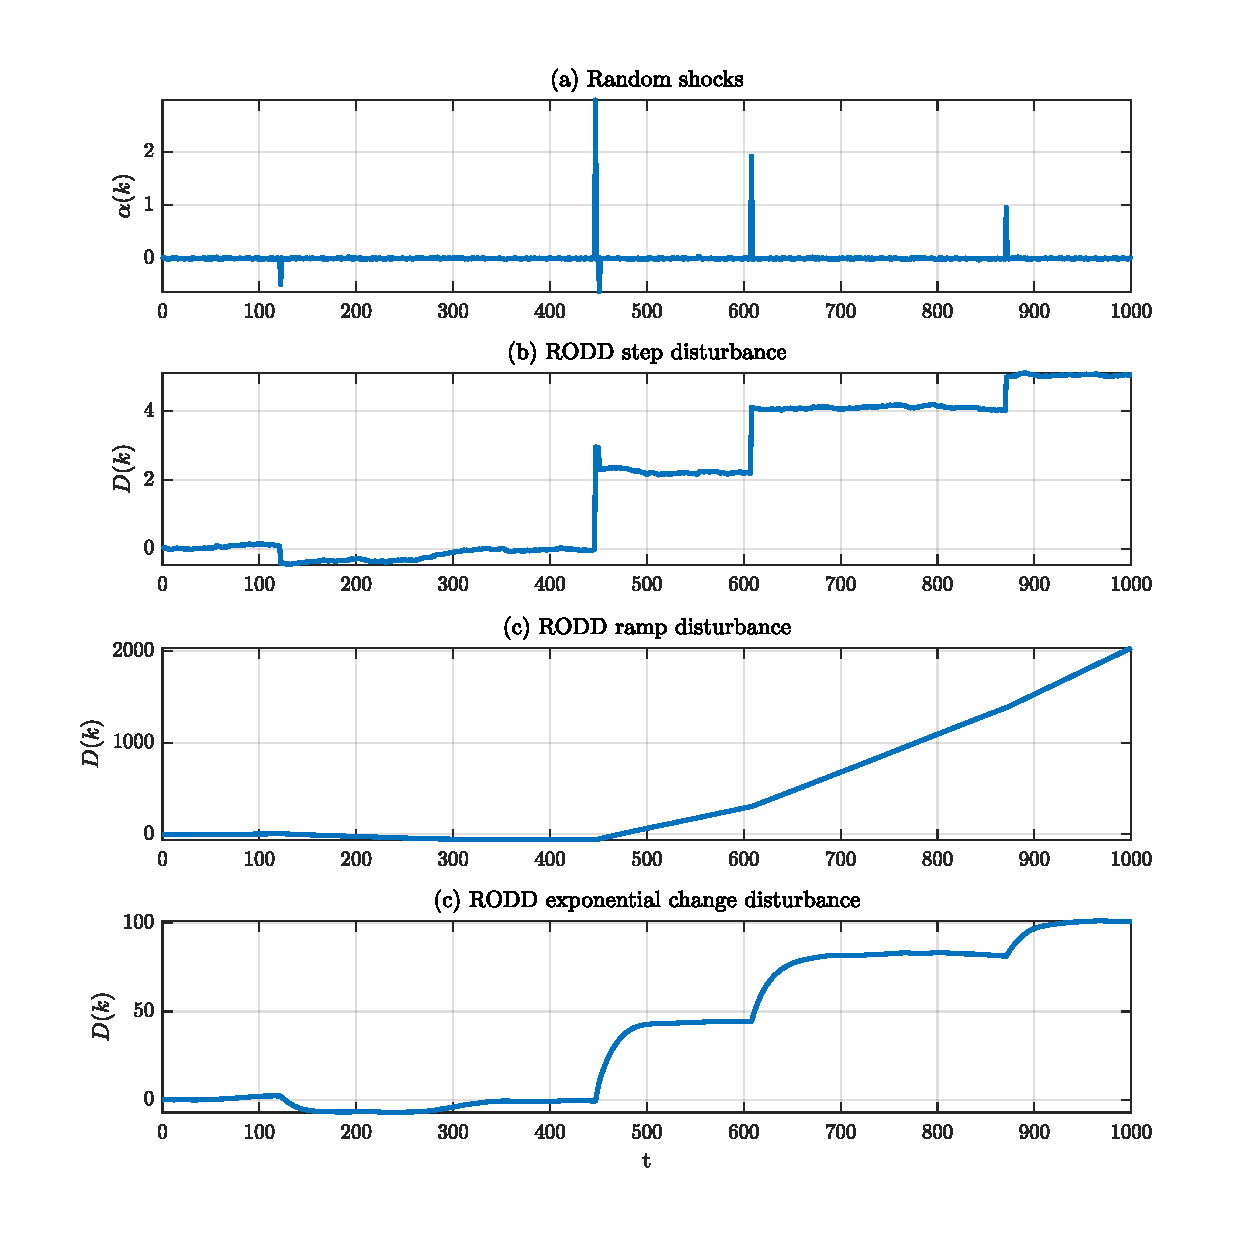
\includegraphics[width=15cm]{images/rodd-sim-plots.pdf}
	\caption{Examples of RODD disturbances}
	\label{fig:rodd-sim-plots}
\end{figure}


\section{Estimating RODD disturbances}

\begin{itemize}
	\item Describe SISO linear system with RODD step disturbance at input
	\item Fig. \ref{fig:sim-sys-diag-siso}: Functional diagram of simulated system
	\item Tuning of different single Kalman filters
	\item Tuning of sequence fusion (Robertson) and sequence pruning (Eriksson and Isaksson) sub-optimal methods
	\item Summary table of observer parameters
	\item Figure: input-output data from simulated system
	\item Figure: observer estimates compared to true output and true system state
	\item Cumulative error plots to compare observers
	\item Waterfall plots of observer internal variables—p(Gamma|Y), K, trace(P)
	\item Table comparing simulation results and metrics
	\item Compare and contrast
	\item Conclude on pros, cons of each and decision to use sequence pruning approach (Eriksson and Isaksson).
\end{itemize}

\begin{itemize}
	\item Include results with 2x2 MIMO system?
\end{itemize}

\begin{figure}[htp]
	\centering
	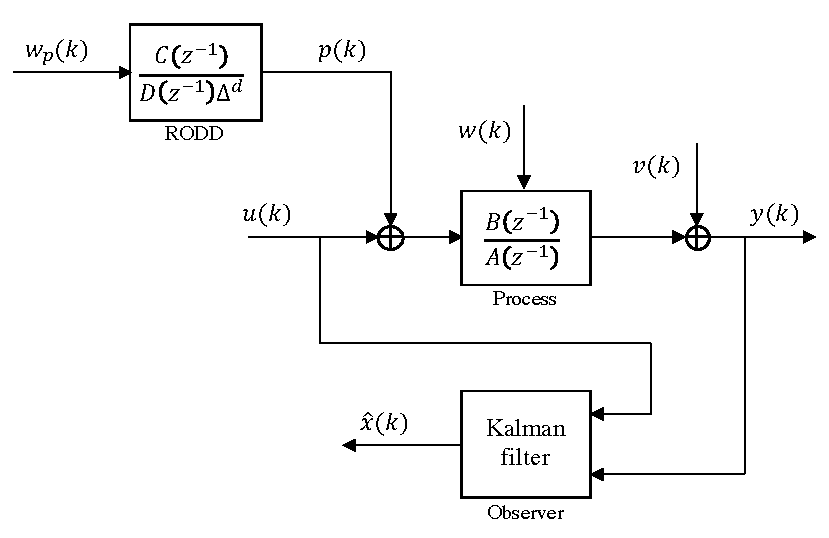
\includegraphics[width=11.5cm]{images/sim-sys-diag-siso.pdf}
	\caption{Functional diagram of the simulated system with observer}
	\label{fig:sim-sys-diag-siso}
\end{figure}

\section{Grinding model simulations}

\begin{itemize}
	\item Unlike previous simulations, this is a non-linear model.
	\item Describe simulations with grinding simulation model (IFAC paper), ore feed changes etc.
	\item Use best observer from previous section (AFMM).
	\item Figure: Input-output data
	\item Figure: comparison of observer estimates
	\item Include sensitivity analysis - model errors, observer (RODD) parameters.
	\item Discuss applications and potential benefits (e.g. RTO).
\end{itemize}

\section{Control performance}

\begin{itemize}
	\item Grinding simulation model in closed loop with MPC controller.
	\item Diagram of feedback system – Figure \ref{fig:sim-mpc-diag}
	\item Table of results - Performance metrics — e.g. tracking error.
	\item Robustness?  E.g. stability margins.
\end{itemize}

\begin{figure}[htp]
	\centering
	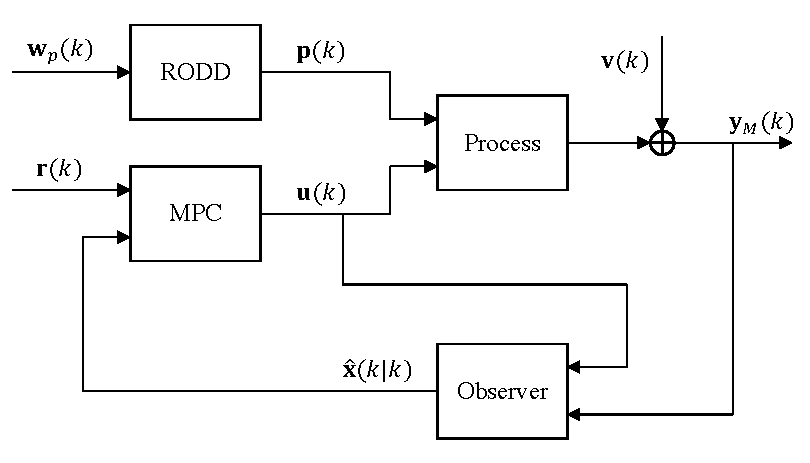
\includegraphics[width=10.5cm]{images/sim-mpc-diag.pdf}
	\caption{Functional diagram of the simulated feedback control system}
	\label{fig:sim-mpc-diag}
\end{figure}